\begin{figure}[htbp]
    \centering
    % --- CASO 1: MOVIMENTO PROGRESSIVO ---
    \begin{subfigure}[b]{0.48\textwidth}
        \centering
        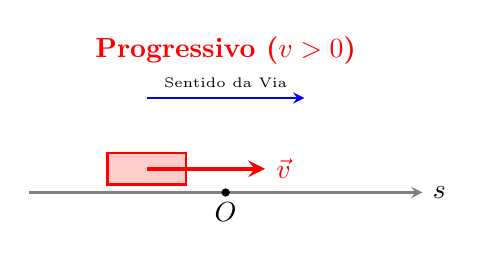
\begin{tikzpicture}[>=stealth]
            % Eixo da trajetória
            \draw[->, thick, gray] (-2.5,0) -- (2.5,0) node[right, black] {$s$};
            \fill (0,0) circle (1.5pt) node[below] {$O$};
            
            % Sentido Positivo da Via
            \draw[->, blue, thick] (-1, 1.2) -- (1, 1.2) node[midway, above, black] {\tiny Sentido da Via};
            
            % O Móvel (Progressivo)
            \draw[fill=red!20, draw=red, thick] (-1.5, 0.1) rectangle (-0.5, 0.5);
            \draw[->, red, ultra thick] (-1, 0.3) -- (0.5, 0.3) node[right] {$\vec{v}$};
            
            \node[red, font=\bfseries] at (0, 1.8) {Progressivo ($v > 0$)};
        \end{tikzpicture}
        \caption{Mesmo sentido da trajetória.}
    \end{subfigure}
    \hfill % Este comando joga o próximo desenho para a outra ponta
    % --- CASO 2: MOVIMENTO RETRÓGRADO ---
    \begin{subfigure}[b]{0.48\textwidth}
        \centering
        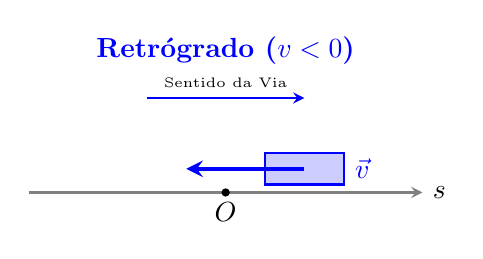
\begin{tikzpicture}[>=stealth]
            % Eixo da trajetória
            \draw[->, thick, gray] (-2.5,0) -- (2.5,0) node[right, black] {$s$};
            \fill (0,0) circle (1.5pt) node[below] {$O$};
            
            % Sentido Positivo da Via
            \draw[->, blue, thick] (-1, 1.2) -- (1, 1.2) node[midway, above, black] {\tiny Sentido da Via};
            
            % O Móvel (Retrógrado)
            \draw[fill=blue!20, draw=blue, thick] (0.5, 0.1) rectangle (1.5, 0.5);
            \draw[<-, blue, ultra thick] (-0.5, 0.3) -- (1, 0.3) node[right, xshift=0.5cm] {$\vec{v}$};
            
            \node[blue, font=\bfseries] at (0, 1.8) {Retrógrado ($v < 0$)};
        \end{tikzpicture}
        \caption{Sentido oposto à trajetória.}
    \end{subfigure}

    \vspace{0.5cm}
    \caption{Classificação do sentido do movimento em relação à orientação da trajetória.}
    \label{fig:progressivo_retrogrado}
\end{figure}
